\documentclass{beamer}
\usepackage{amsmath}
\usepackage{mathtools}
\usepackage{multimedia}
\usepackage[outline]{contour}

\mode<presentation>
{
  \useoutertheme{default}
}

\beamertemplatenavigationsymbolsempty
\setbeamertemplate{frametitle}[default][center]
%\setbeamercolor{frametitle}{fg=white}
%\setbeamercolor{background canvas}{bg=black}
%\setbeamercolor{normal text}{fg=white}
%\usepackage[dvipsnames]{xcolor}
\definecolor{cyan}{rgb}{0,1,1}
\definecolor{yellow}{rgb}{1,1,0}
\definecolor{magenta}{rgb}{1,0,1}

\title{Tumours, risk, and waves: learning from multi-modal data to predict
outcomes in \emph{NF2} schwannomatosis}
\author{Chay Paterson}
\institute{University of Manchester}
\date{July 13, 2026}

\begin{document}

\frame{\titlepage}

% this minisympsosium emphasises translational stuff, so start with the
% schwannomatosis project and applications to tmt protocols

\begin{frame}
    \frametitle{Where I am and what I do}
    % talk about manchester, me, infrastructure, network -- first slide, intro!
        % one side gives me lots of clinical data: ages, dates, outcomes, FBCs, etc.
    \begin{columns}
        \begin{column}{0.3\textwidth}
        Smith Lab (Manchester Royal Infirmary) $\rightarrow$

        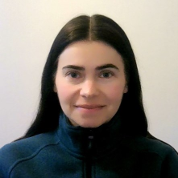
\includegraphics[width=1.0\textwidth]{../figures/Miriam.png}

        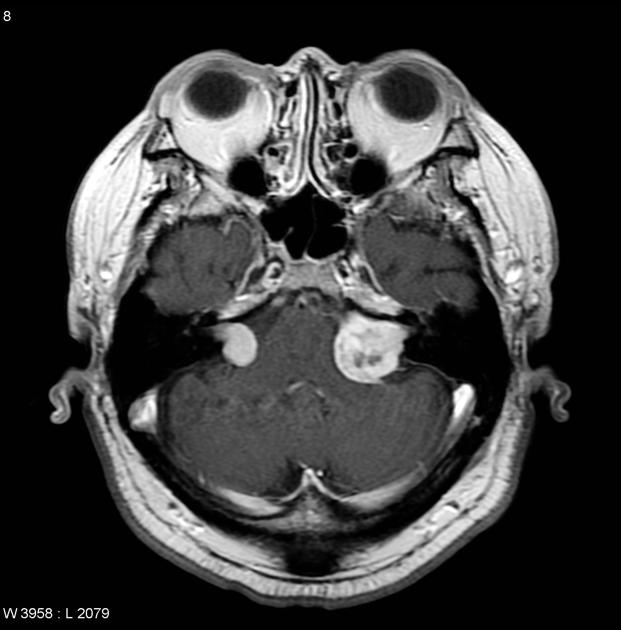
\includegraphics[width=0.8\textwidth]{../figures/nf2-2467429117.jpg}

        \;

        
\includegraphics[width=1.0\textwidth]{../figures/MFT-logo}

        \end{column}
        \begin{column}{0.4\textwidth}
         My modelling group (University of Manchester)

        
\includegraphics[width=1.0\textwidth]{../figures/Banff.jpg}

            \begin{columns}
            \begin{column}{0.5\textwidth}
            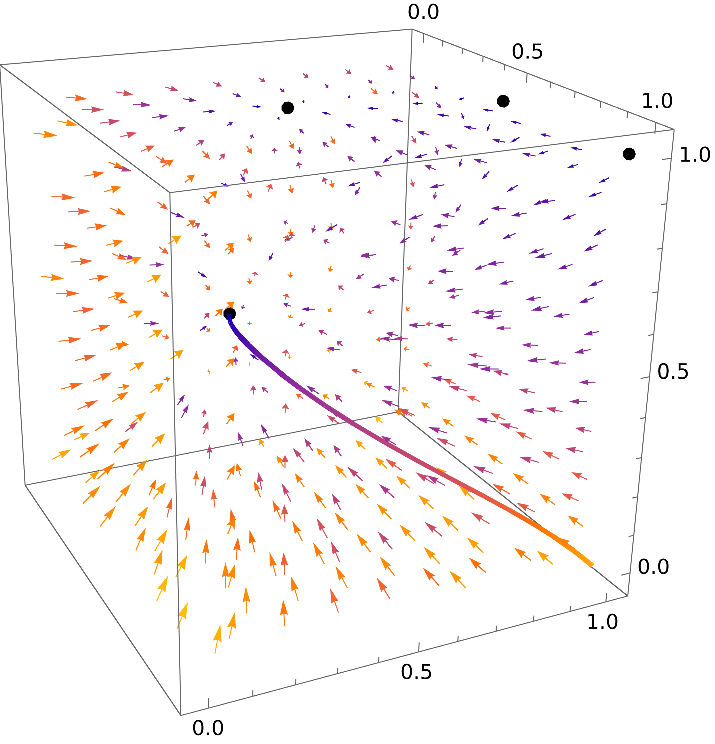
\includegraphics[width=1.0\textwidth]{../figures/flowcube1}
            \end{column}
            \begin{column}{0.5\textwidth}
            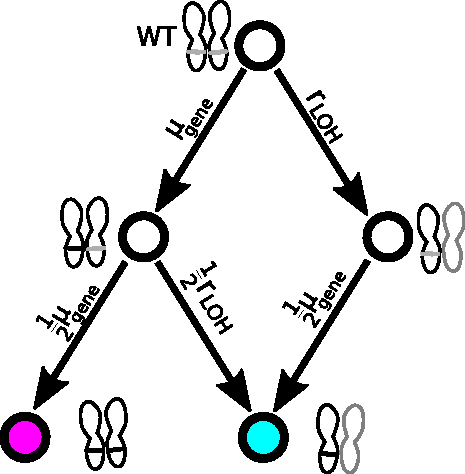
\includegraphics[width=1.0\textwidth]{../figures/diagram4c}
            \end{column}
            \end{columns}

        \;

        
\includegraphics[width=1.0\textwidth]{../figures/cdmrp_logo_03.png}

        \end{column}
        \begin{column}{0.3\textwidth}
         $\leftarrow$ Wedge Lab and Jamie Weaver's group (The Christie/MCRC)

        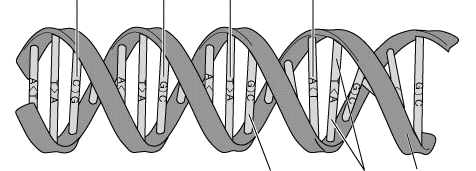
\includegraphics[width=1.0\textwidth]{../figures/dna.png}
        
\includegraphics[width=1.0\textwidth]{../figures/David.png}

        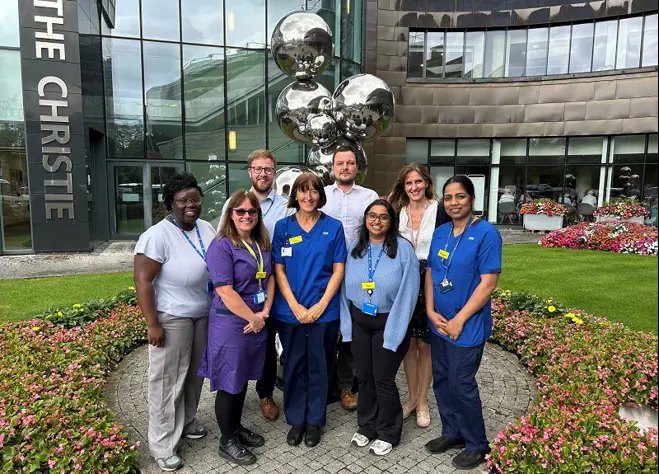
\includegraphics[width=1.0\textwidth]{../figures/pan-tumour-research-team.png}

        \;

        
        \end{column}
    \end{columns}
        % one side gives me lots of WGS data (various callers on whole genomes)
        % two modalities, matched to each Pt! 
\end{frame}

% animation: overlay image
\begin{frame}
    \frametitle{Where I am and what I do}
    % talk about manchester, me, infrastructure, network -- first slide, intro!
        % one side gives me lots of clinical data: ages, dates, outcomes, FBCs, etc.
    \begin{columns}
        \begin{column}{0.3\textwidth}
        Smith Lab (Manchester Royal Infirmary) $\rightarrow$

        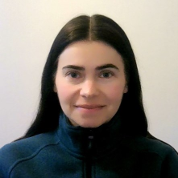
\includegraphics[width=1.0\textwidth]{../figures/Miriam.png}

        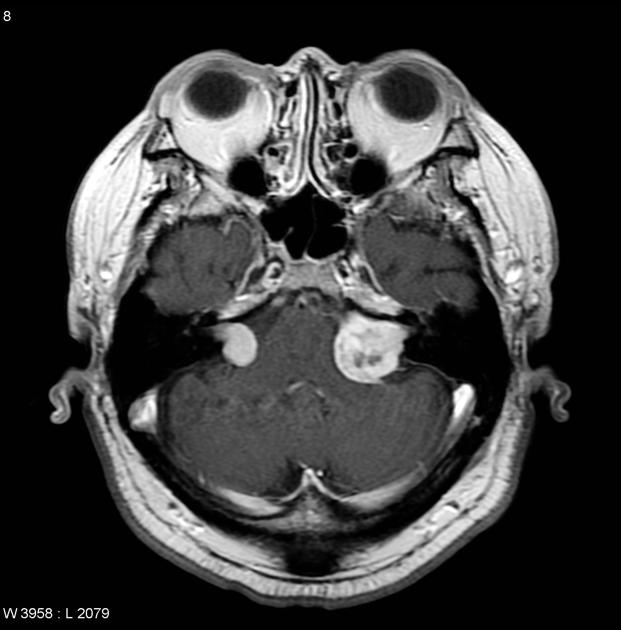
\includegraphics[width=0.8\textwidth]{../figures/nf2-2467429117.jpg}

        \;

        
\includegraphics[width=1.0\textwidth]{../figures/MFT-logo}

        \end{column}
        \begin{column}{0.4\textwidth}
         My modelling group (University of Manchester)

        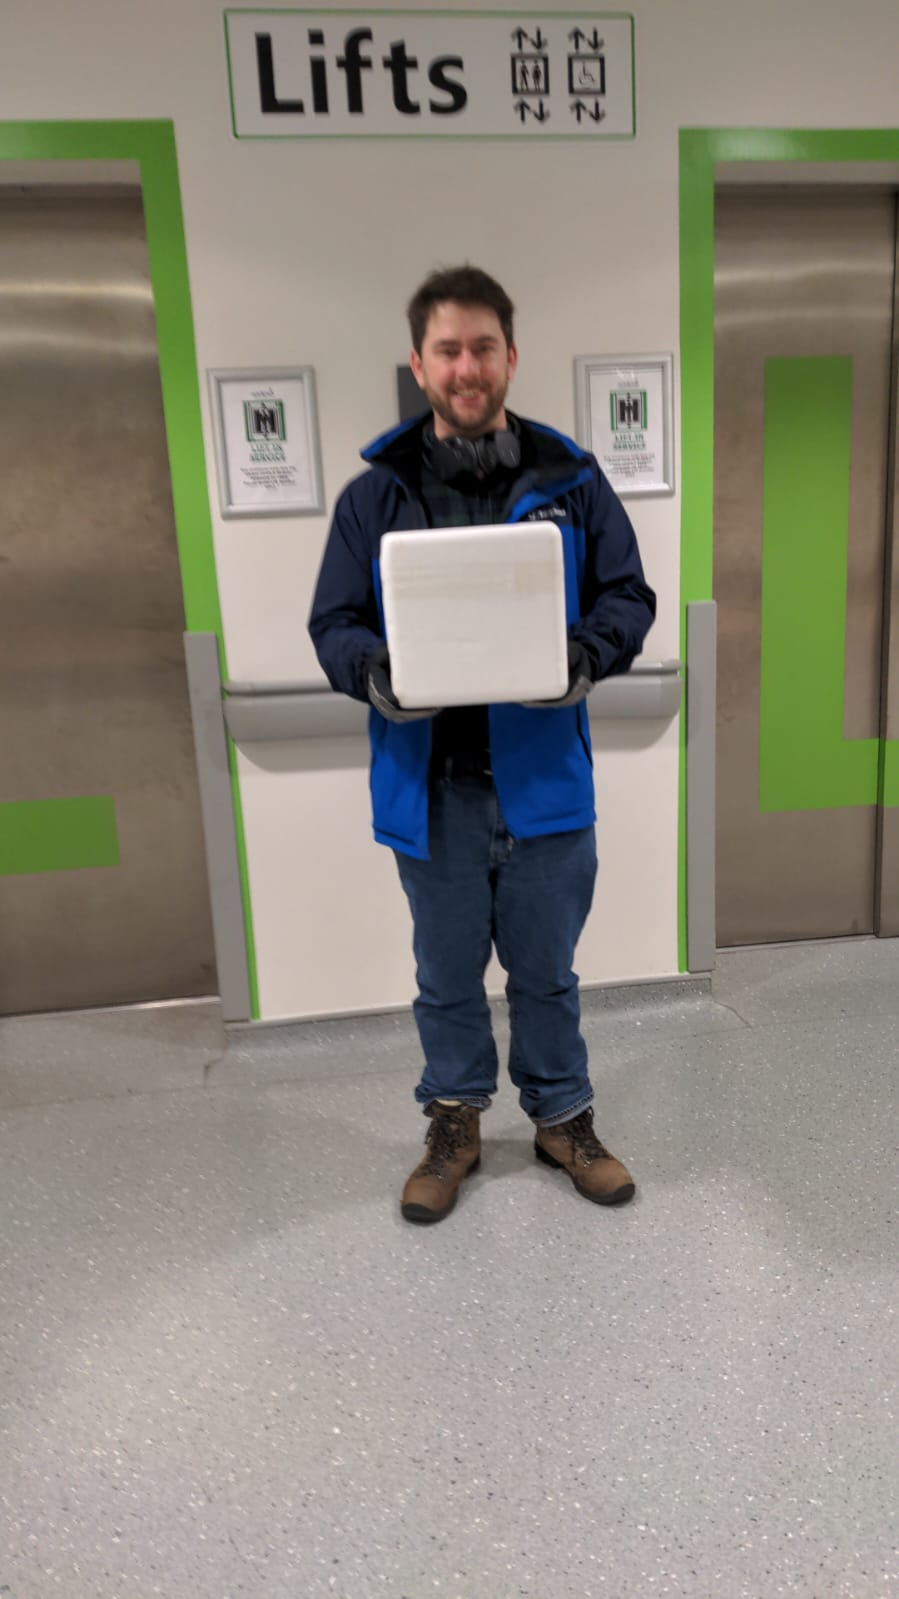
\includegraphics[width=1.0\textwidth]{../figures/metumours.jpg}

            \begin{columns}
            \begin{column}{0.5\textwidth}
            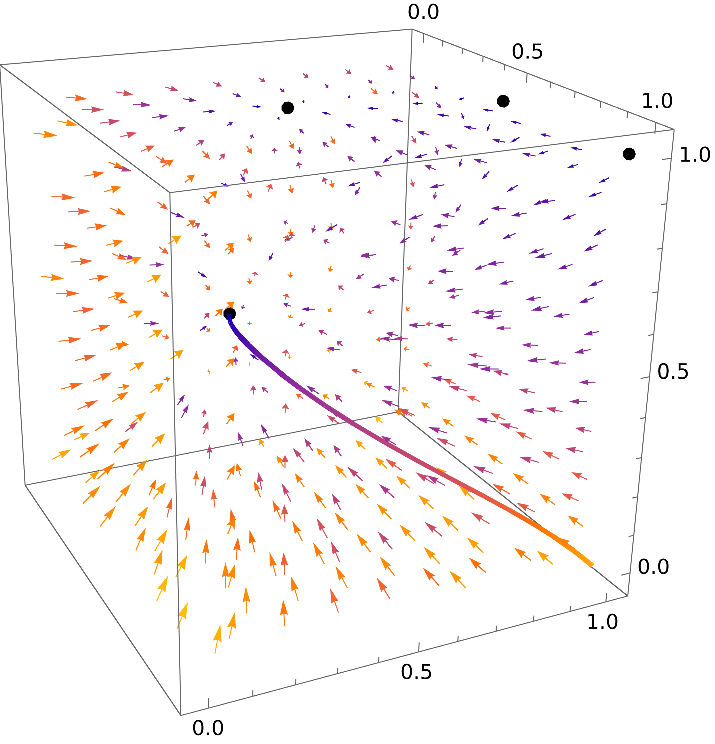
\includegraphics[width=1.0\textwidth]{../figures/flowcube1}
            \end{column}
            \begin{column}{0.5\textwidth}
            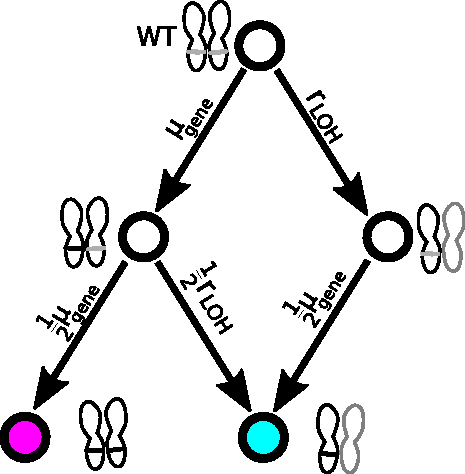
\includegraphics[width=1.0\textwidth]{../figures/diagram4c}
            \end{column}
            \end{columns}

        \;

        
\includegraphics[width=1.0\textwidth]{../figures/cdmrp_logo_03.png}

        \end{column}
        \begin{column}{0.3\textwidth}
         $\leftarrow$ Wedge Lab and Jamie Weaver's group (The Christie/MCRC)

        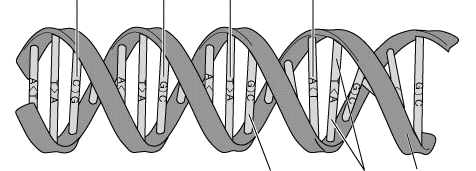
\includegraphics[width=1.0\textwidth]{../figures/dna.png}
        
\includegraphics[width=1.0\textwidth]{../figures/David.png}

        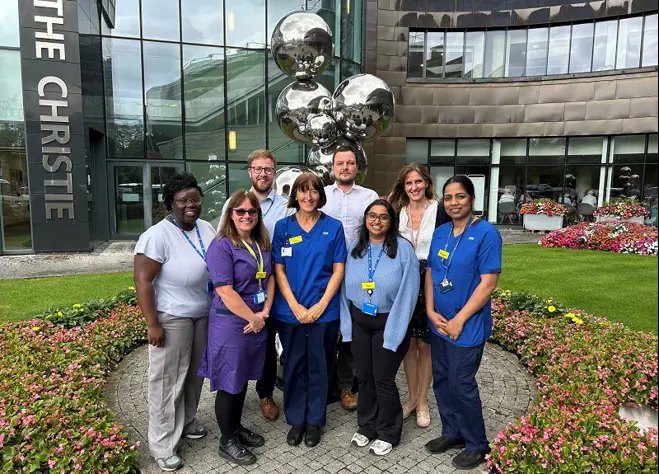
\includegraphics[width=1.0\textwidth]{../figures/pan-tumour-research-team.png}

        \;

        
        \end{column}
    \end{columns}
        % one side gives me lots of WGS data (various callers on whole genomes)
        % two modalities, matched to each Pt! 
\end{frame}



% second slide: the radiotherapy study and core findings

\begin{frame}
    \frametitle{Schwannomatosis and radiotherapy}
    \begin{columns}
        \begin{column}{0.5\textwidth}
        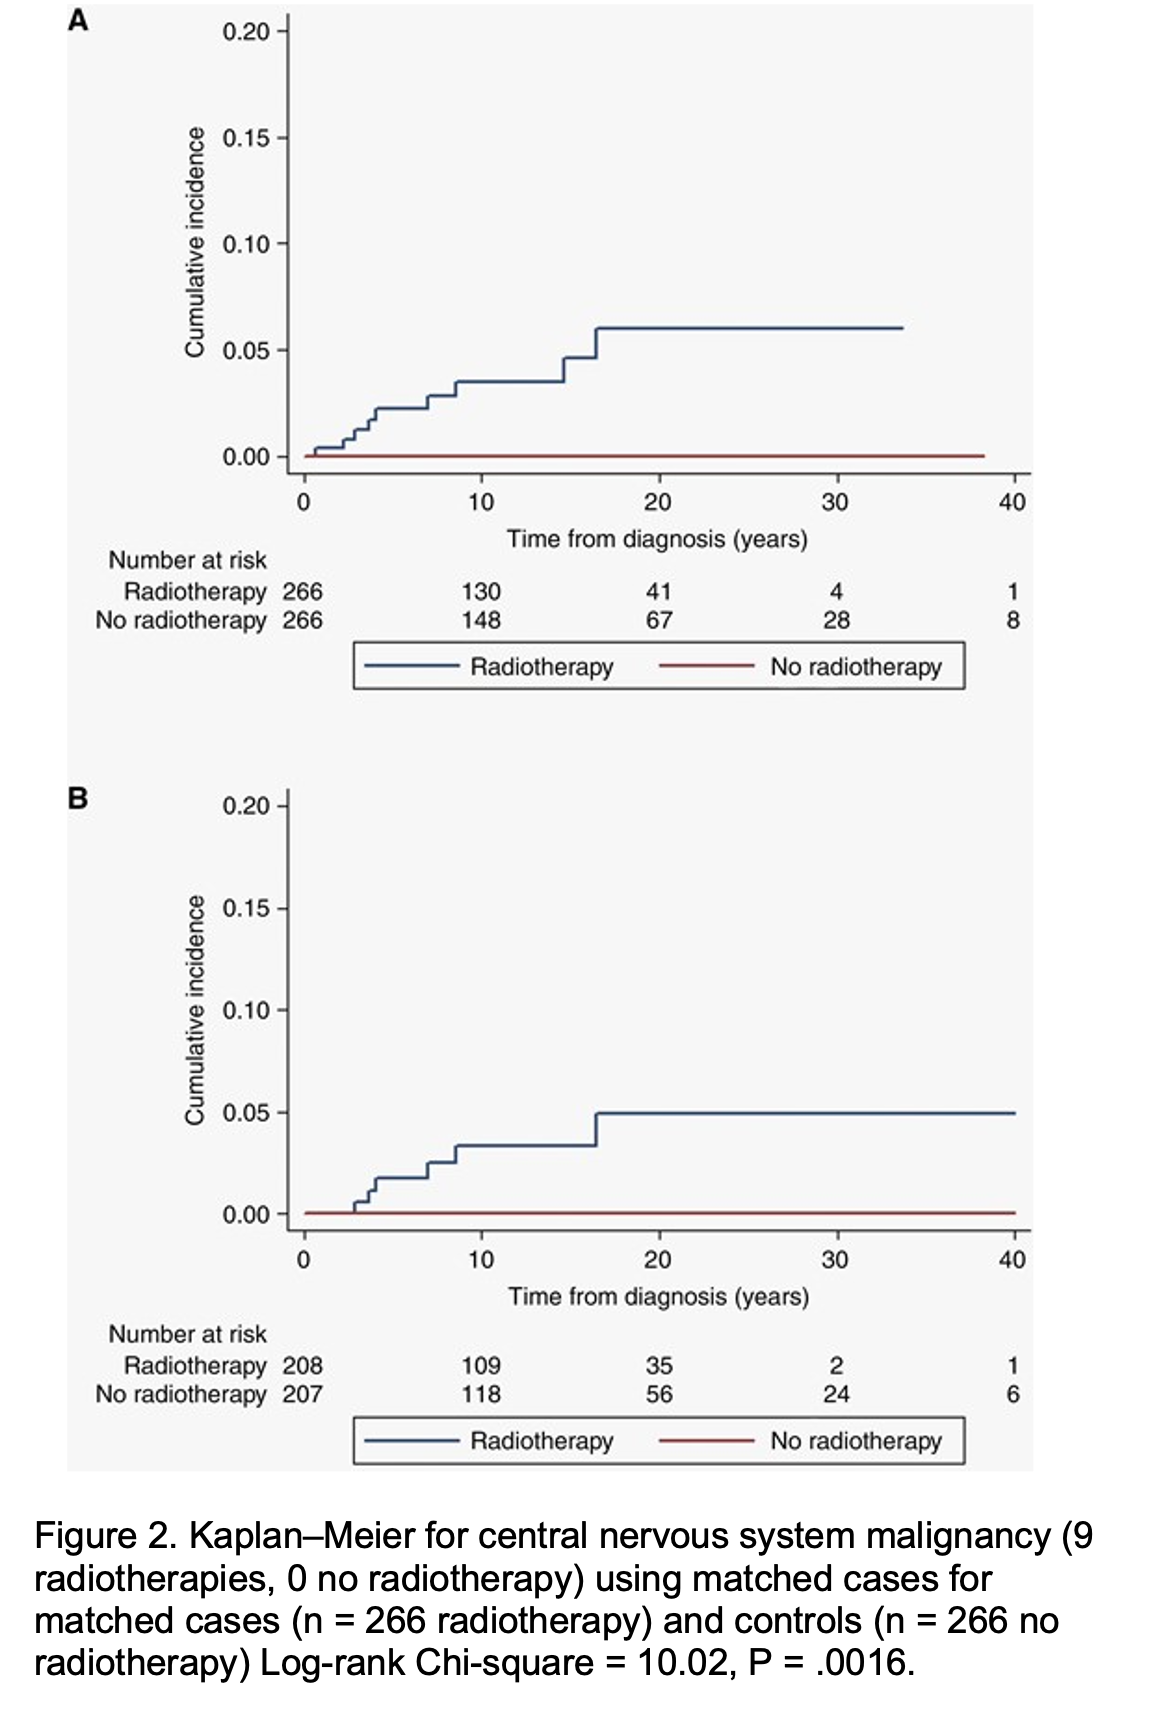
\includegraphics[width=1.0\textwidth]{../figures/recurrence_rad_2024.png}
        \end{column}
        \begin{column}{0.5\textwidth}
        \begin{itemize}
            \item Complication: secondary CNS/skull base malignancies
            \item Excess absolute risk of $5\%$
            \item Relative risk more than $10\times$ general pop
            \item (Conditional) mean recurrence time $6y$
        \end{itemize}

        \;

        ``NF2 patients should not be offered radiotherapy as first-line treatment of benign tumors and should be given a frank discussion of the potential 5\% excess absolute risk of M/MP.''${}^1$
        \end{column}
    \end{columns}


\includegraphics[width=0.5\textwidth]{../figures/NIHR-MBRC-logo}

\footnotetext[1]{Gareth Evans et al., Neuro-Oncology Advances, Volume 5, Issue 1, January-December 2023, vdad025}
\end{frame}

% "i am trying to understand why this happens..."
% basic problem is to integrate the clinical data

% third slide with (proposed) pipeline.

\begin{frame}
    \frametitle{Idealised pipeline for multimodal data integration}

    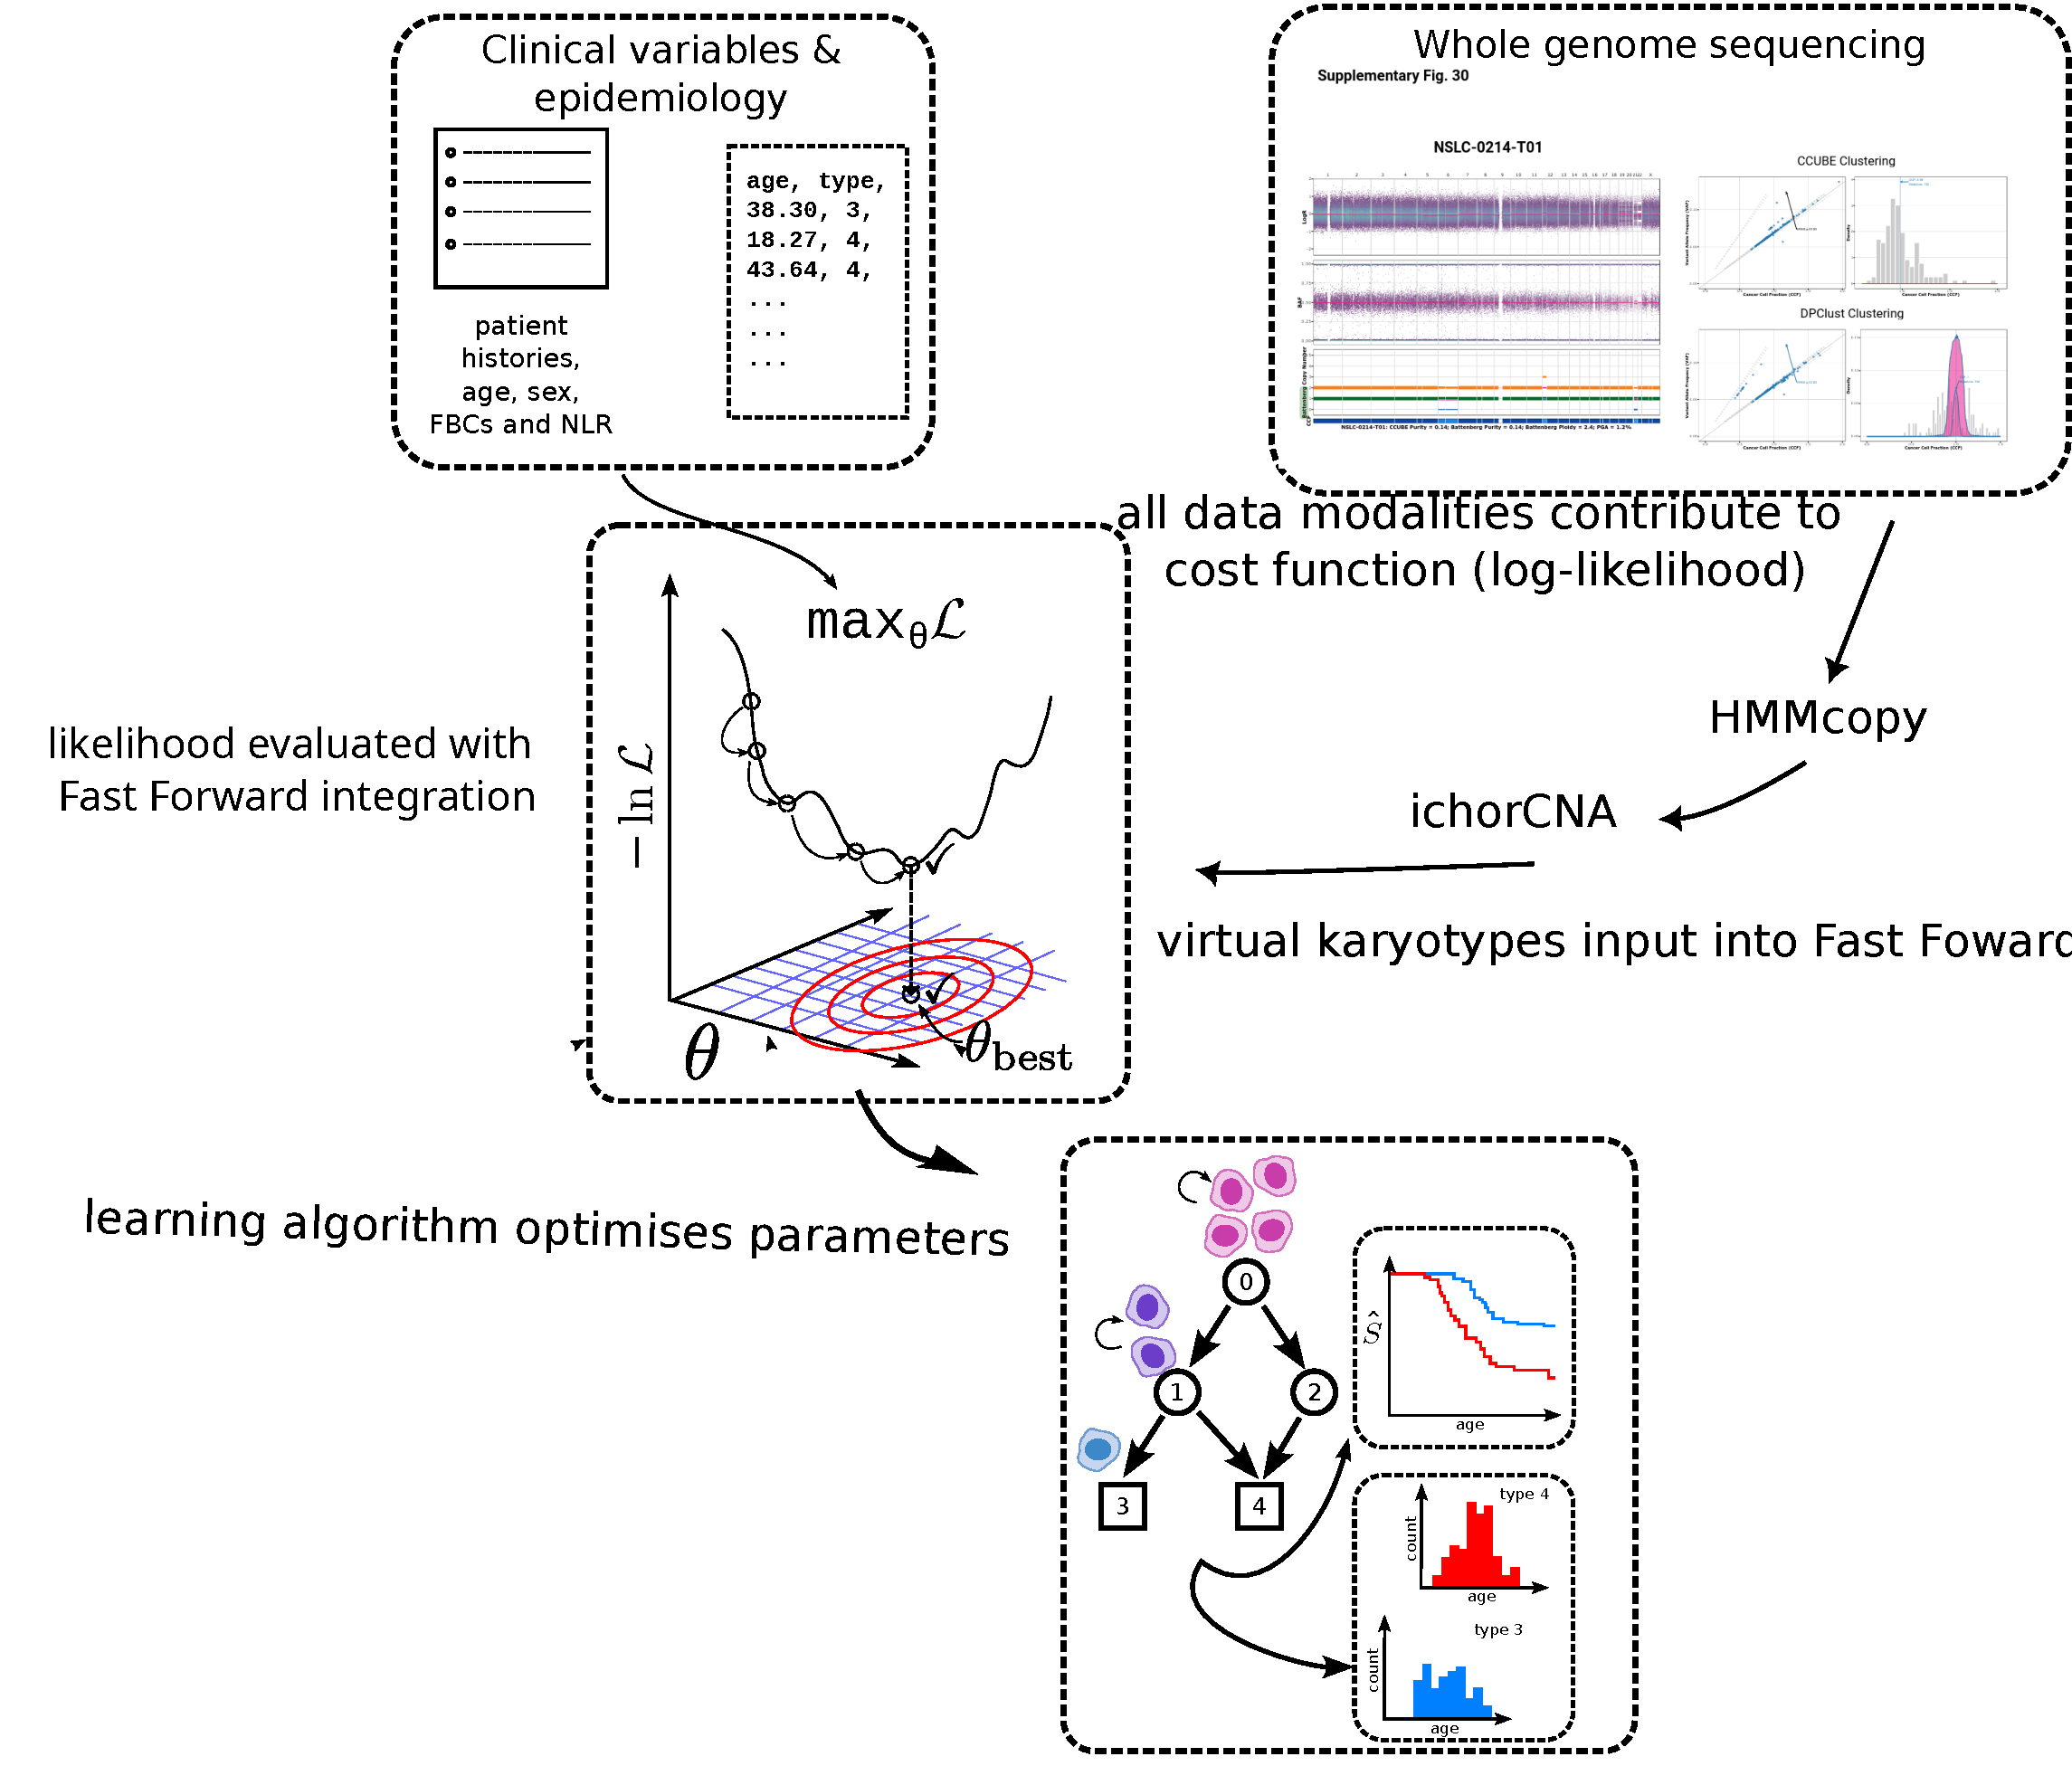
\includegraphics[width=0.8\textwidth]{../figures/bimodal_flowchart}

    The problem is that existing models are not general enough to include both
    modalities (in a nontrivial likelihood function)
\end{frame}
% "the basic problem here is that existing models for either modality are not
% general enough to include both, which is necessary to learn from both
% modalities simultaneously."

% then some methods:

\begin{frame}
    \frametitle{A brief history of multi-stage clonal expansion theory}

    \begin{columns}
        \begin{column}{0.6\textwidth}
        This network...
        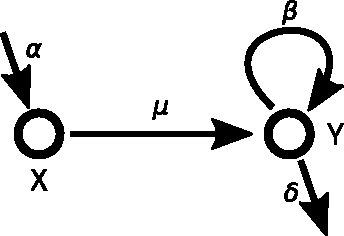
\includegraphics[width=\textwidth]{../figures/diagram1}
        \end{column}
        \begin{column}{0.4\textwidth}
        corresponds to this stochastic process:...
        \begin{align}
            \emptyset \rightarrow X, &\qquad \mathrm{rate\;}\alpha
            \nonumber \\
            % NB
            X \rightarrow X + Y, &\qquad\mathrm{rate\;}\mu X
            \nonumber \\
            Y \rightarrow Y + Y, &\qquad\mathrm{rate\;} \beta Y
            \nonumber \\
            Y \rightarrow \emptyset, &\qquad\mathrm{rate\;} \delta Y
            \nonumber
        \end{align}
        \end{column}
    \end{columns}
\footnotetext[1]{C. Paterson, I. Bozic, H. Clevers, PNAS 2020; 117(34): 20681-20688}
\end{frame}

\begin{frame}
    \frametitle{A brief history of multi-stage clonal expansion theory}
    \framesubtitle{P. Armitage and R. Doll\footnotemark[12]}

    \begin{columns}
        \begin{column}{0.5\textwidth}
        
\includegraphics[width=\textwidth]{../figures/LSHTM-small.jpg}
        \end{column}
        \begin{column}{0.5\textwidth}
        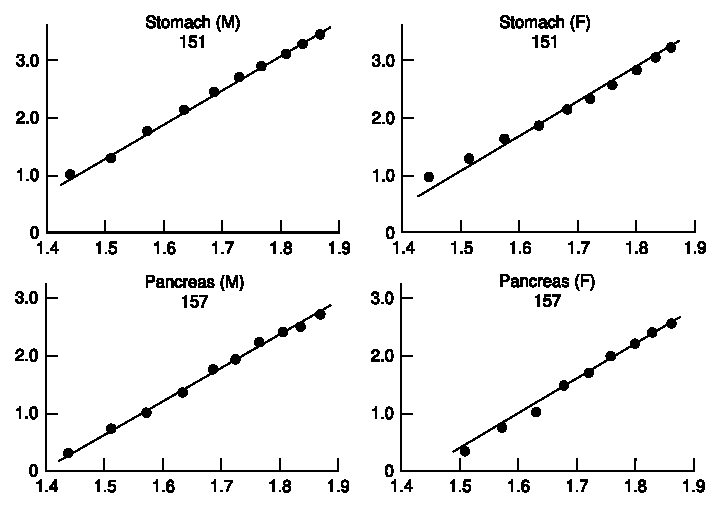
\includegraphics[width=\textwidth]{../figures/PArmitageRDoll_1954_6602297.pdf}
        \end{column}
    \end{columns}


\footnotetext[1]{P. Armitage and R. Doll, British Journal of Cancer 1954; 8: 1–12}
\footnotetext[2]{P. Armitage and R. Doll, British Journal of Cancer 1957; 11(2): 161-169}
\end{frame}

\begin{frame}
    \frametitle{A brief history of multi-stage clonal expansion theory}
    \framesubtitle{A.G. Knudson\footnotemark[12]}

    \begin{columns}
        \begin{column}{0.5\textwidth}
            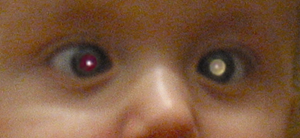
\includegraphics[width=0.90\textwidth]{../figures/Rb_whiteeye.PNG}
            \;
            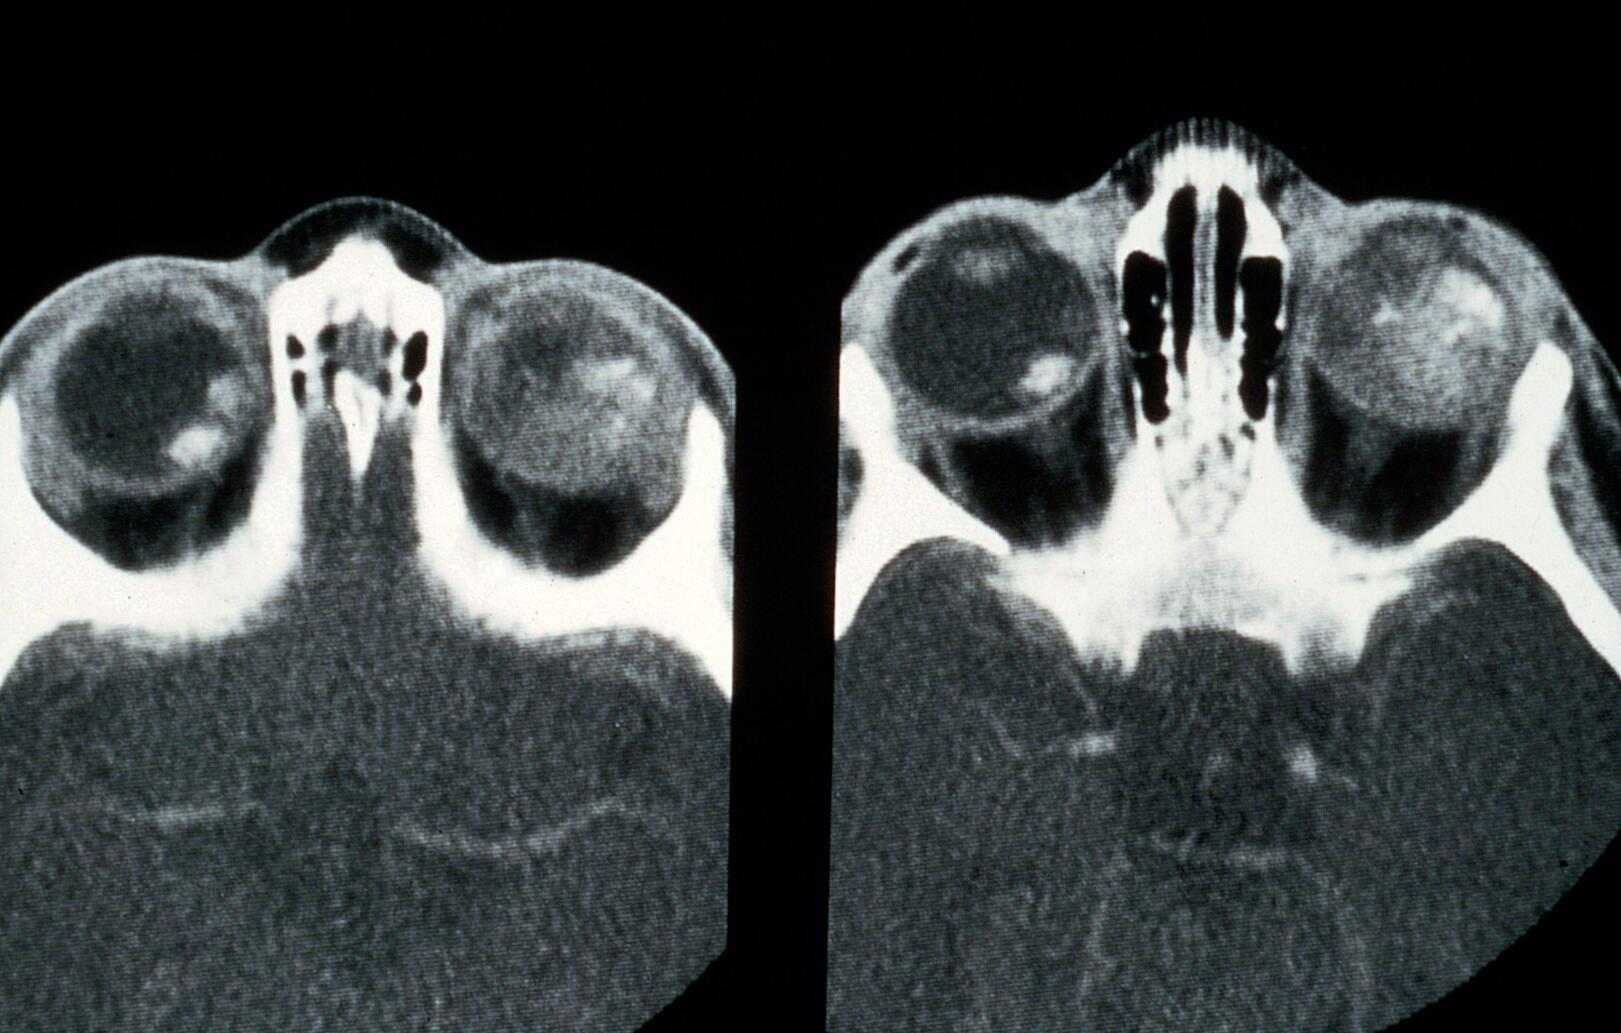
\includegraphics[width=0.90\textwidth]{../figures/retinoblastoma.jpg}
        \end{column}
        \begin{column}{0.5\textwidth}
            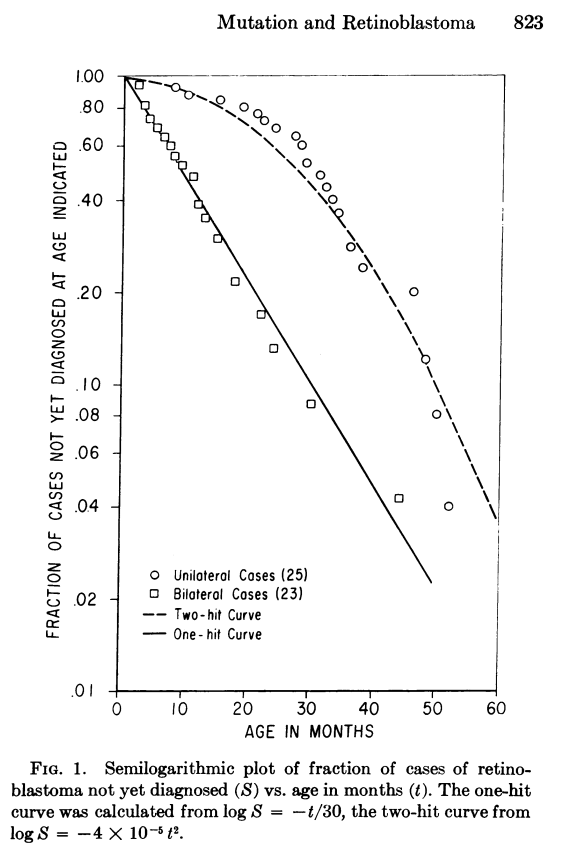
\includegraphics[width=0.90\textwidth]{../figures/Screenshot_2022-10-31_11-57-01.png}
        \end{column}
    \end{columns}

\footnotetext[1]{AG. Knudson, PNAS 68.4 (1971): 820-823.}
\footnotetext[2]{F. Michor, Y. Iwasa and MA. Nowak, Nature Reviews Cancer 2004; 4: 197-205 doi:10.1038/nrc1295}
\end{frame}

\begin{frame}
    \frametitle{How do these studies work?}

    What are the relevant observables in this type of longitudinal study \& data
    analysis? 

    Track a cohort that initially contains $N$ patients in the study:

    \begin{itemize}
        \item Age-specific incidence $I(a)$: rate at which new cases are
        recorded in the cohort with ages between $a$ and $a + da$
        \item Diagnosis-free survival function $S(a)$: probability to survive to age $a$ without being diagnosed.
    \end{itemize}

    \begin{equation}
        I(a) = -N \frac{dS}{da} = -N\; S(a) \frac{d \ln S}{da}
    \end{equation}
\end{frame}

\begin{frame}
    \frametitle{So what?}

    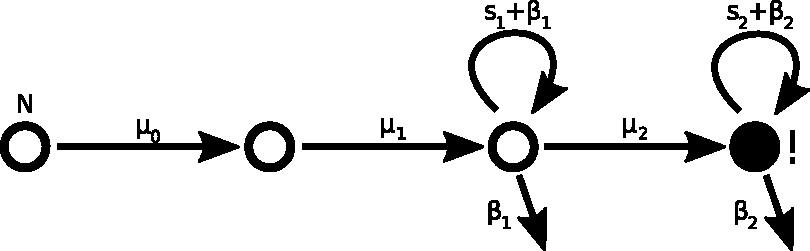
\includegraphics[width=1.00\textwidth]{../figures/diagram3}

    \begin{itemize}
        \item The survival curve $S(a)$ determines the incidence curve $I(a)$ 
        \item The model determines the survival curve: the probability not to
        end up at one of the end nodes of the graph. We want to know what model+parameters best agree with
        data from studies.
        \item To fit (or ``train'') the model to longitudinal data, we need to compute $S(a)$!
    \end{itemize}

    This is the central mathematical problem in cancer epidemiology. \emph{How do we compute $S$?}
\end{frame}

\begin{frame}
    \frametitle{Models on graphs}
    \begin{columns}
        \begin{column}{0.5\textwidth}
        \begin{enumerate}
            \item Most methods for computing $S(a)$ do not consider graphs with
            multiple end nodes
            \item To study \textbf{specific genes} and mechanisms of interest
            (SNVs, LOH, CNA, etc.), we need to evaluate $S(a)$ for a model
            defined on a graph (right)
        \end{enumerate}
        \end{column}
        \begin{column}{0.5\textwidth}
        \begin{center}
            \small{example model}
        \end{center}
            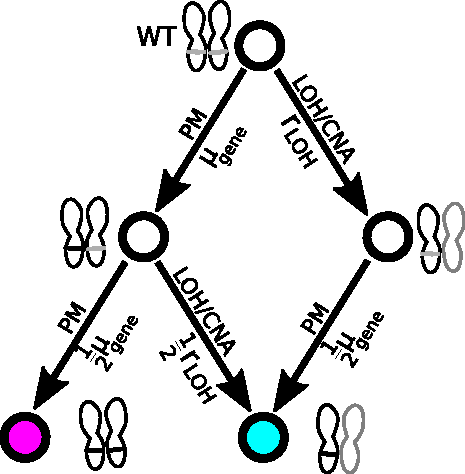
\includegraphics[width=\textwidth]{../figures/diagram4}
        \end{column}
    \end{columns}

    \begin{center}
        This gets us the incidence of \emph{specific genomic subtypes} 
    \end{center}
\end{frame}

\begin{frame}
    \frametitle{Colorectal adenocarcinoma model}
    \begin{columns}
        \begin{column}{0.5\textwidth}
        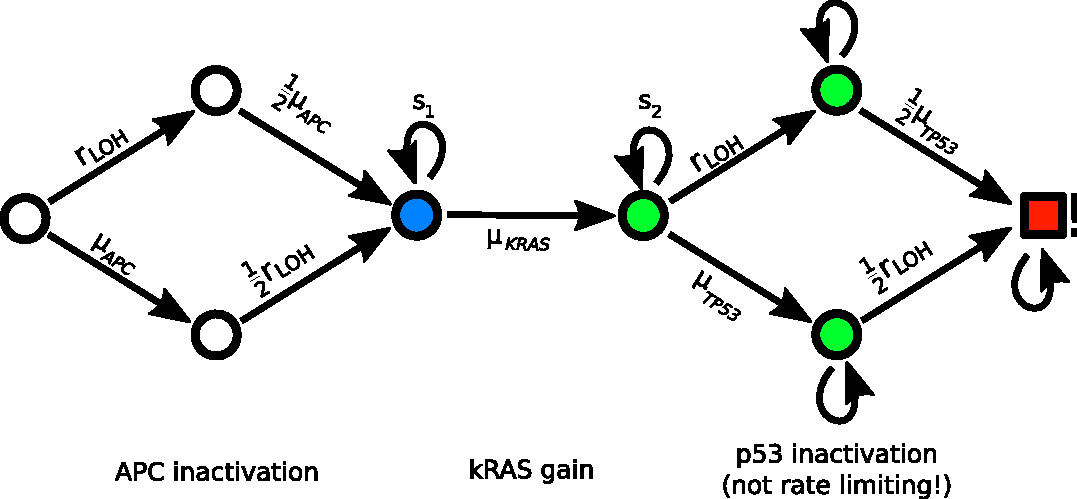
\includegraphics[width=1.0\textwidth]{../figures/diagram7}
        \begin{itemize}
            \item Can use A-D type approximation, or stochastic simulations
            \item Conditional path probabilities $P(X_i)$ encode fitnesses
        \end{itemize}
        but:
        \begin{itemize}
            \item Mean-field breaks down at old ages / large probabilities
            \item Stochastic simulations are \emph{extremely slow}
            \item 
        \end{itemize}
        \end{column}
        \begin{column}{0.5\textwidth}
        % graph from our PNAS paper
        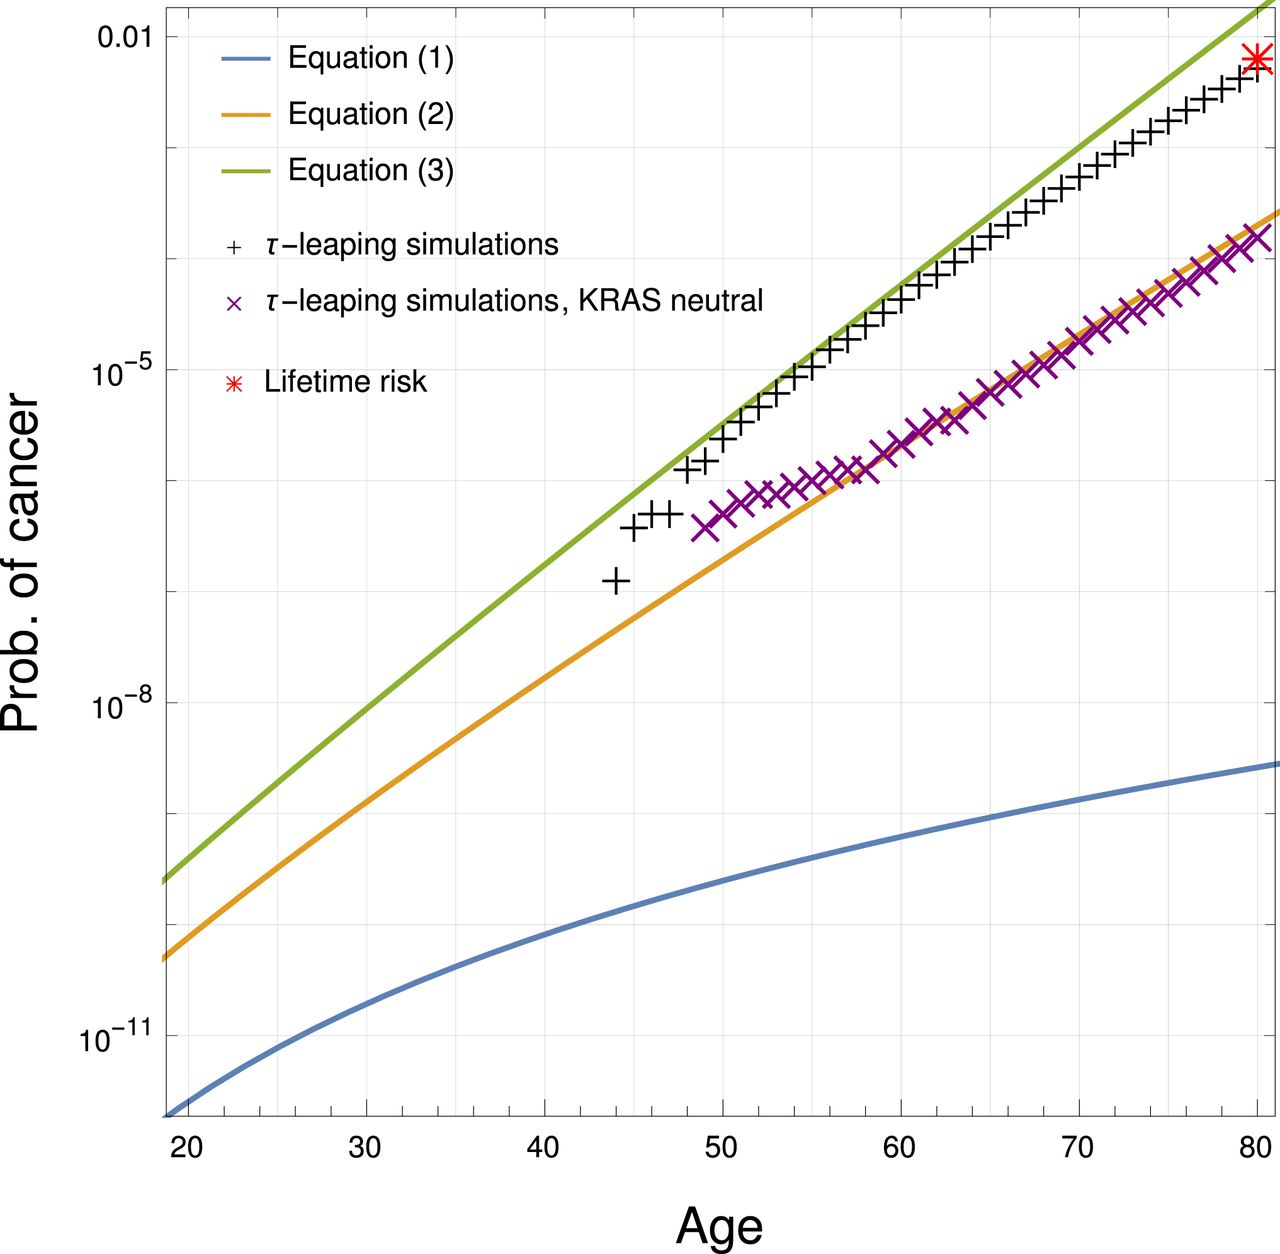
\includegraphics[width=\textwidth]{../figures/F2.large.jpg}
        \end{column}
    \end{columns}

\footnotetext[1]{C. Paterson, I. Bozic, H. Clevers, PNAS 2020; 117(34): 20681-20688}
\end{frame}

\begin{frame}
    \frametitle{Alternative approach: Kolmogorov forward equations}
    Define a more general generating function $\Psi$:

    \begin{equation}
        \Psi(t, \vec{q}) = \mathbb{E}\left[\prod_j q_j^{N_j}\right]
    \end{equation}
    and derive Kolmogorov forward equations instead. Then we can numerically
    integrate these, and get survival curves $S_i(a)$ for different types of
    cancer $i$. E.G. tumours with clonal LOH, or no clonal LOH.

    \begin{equation}
        S_i(a) = \frac{\Psi(a, \vec{q}_F)}{\Psi(a, \vec{q}_{F - i})}
    \end{equation}
    with $F$ end nodes.People knew about this approach for a long time (since 1970s) but it was never
    considered as useful as backward equations.

\footnotetext[1]{SH Moolgavkar and DJ Venzon, Math. biosc. 1979; 47(1): 55-77}
\footnotetext[2]{DW Quinn, Risk Analysis 1989; 9(3): 407-13}
\end{frame}

\begin{frame}
    \frametitle{Kolmogorov forward equations as wave equations}

\begin{center}
        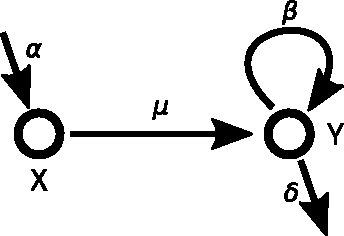
\includegraphics[width=0.4\textwidth]{../figures/diagram1}
\end{center}

    Briefly: the Kolmogorov forward equations in $P(N_0, \dots)$
\begin{align}
    \frac{d P(N_0, N_1, \dots)}{dt} &= \sum_{vertices} \alpha (N_j - 1)
    P(\dots, N_j - 1, \dots) \nonumber \\
    &\; - \alpha N_j P(\dots, N_j, \dots) \nonumber \\
    &\; + \beta \cdots + \mu \cdots + \delta \cdots \nonumber
\end{align}

get transformed...

\end{frame}

\begin{frame}
    \frametitle{Kolmogorov forward equations as wave equations}
    They transform with $P \rightarrow \Psi$:
    \begin{equation}
        \frac{\partial \Psi}{\partial t} = \sum_{vertices} \alpha (q_j - 1) q_j
        \frac{\partial \Psi}{\partial q_j} + \dots = \mathcal{H}\Psi
    \end{equation}
    where $\mathcal{H}$ is a hyperbolic differential operator.

    \;

    Because this is a hyperbolic wave equation, we can solve for future values
    of $\Psi$ if we have initial values, by evolving them along
    characteristics.

\footnotetext[1]{SH Moolgavkar and DJ Venzon, Math. biosc. 1979; 47(1): 55-77}
\end{frame}

\begin{frame}
    \frametitle{Kolmogorov forward equations}

    \begin{columns}
        \begin{column}{0.5\textwidth}
    Using the big generating function $\Psi$, find the corresponding wave
    equation:

    \begin{equation}
        \frac{d \Psi}{ dt} = \mathcal{H} \Psi
    \end{equation}

    This can be solved using the method of characteristics, so we can solve

    \begin{equation}
        \frac{d \vec{\gamma}}{ dt} = \vec{X}
        \label{eq:char}
    \end{equation}
    numerically, using an appropriate time stepper.

    \;

    (NB: \eqref{eq:char} is always a Hamiltonian system too)


        \end{column}
        \begin{column}{0.5\textwidth}
            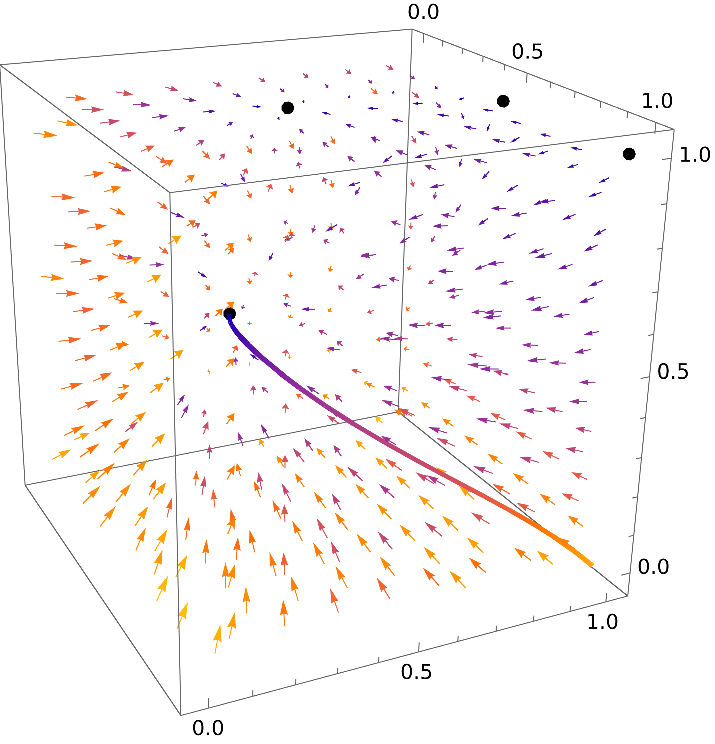
\includegraphics[width=\textwidth]{../figures/flowcube1}

            \;

            The vector field $\vec{X}$ and a characteristic $\vec{\gamma}$
        \end{column}
    \end{columns}
\footnotetext[1]{SH Moolgavkar and DJ Venzon, Math. biosc. 1979; 47(1): 55-77}
\end{frame}

\begin{frame}
    \frametitle{Errors and runtime}

    To estimate $\hat{S}$ to within an error less than chosen $\epsilon$, we
    would need to run $T \propto \epsilon^{-0.5}$ Monte Carlo simulations.

    \;

    What happens with our new method, using a simple Runge-Kutta stepper?

    \begin{equation}
        \epsilon \sim \Delta t^2
    \end{equation}
    and runs in 
    \begin{equation}
        T \sim \Delta t^{-1} \sim \mathcal{O}(\epsilon^{-1/2})
    \end{equation}
    so new runtime $\sim \mathcal{O}\left(\right.$ old runtime
    $\left.^{1/4}\right)$.

    \;

    Amazing!
\end{frame}

\begin{frame}
    \frametitle{Fast forward method}

    \begin{center}
    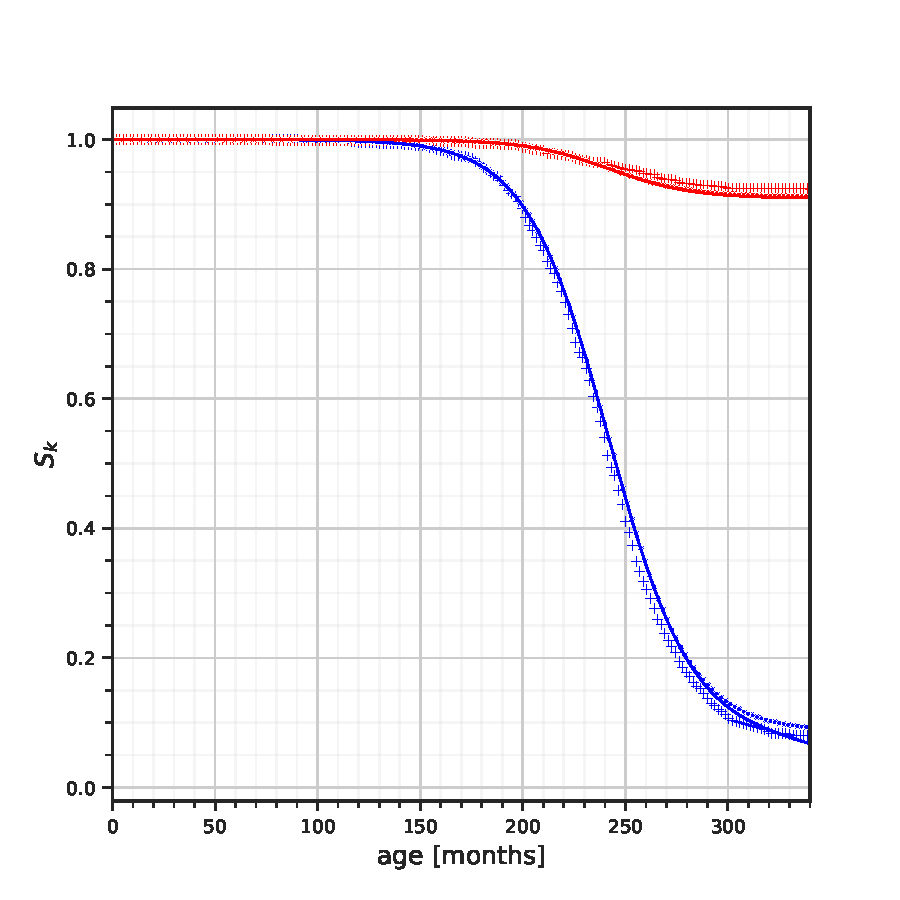
\includegraphics[height=0.8\textheight]{../figures/SCurveComparison.pdf}
    \end{center}

    Random sampling vs fast forward method:

    Monte Carlo: $\approx 5000$s
    Fast forward: 4ms
\end{frame}

\begin{frame}
    \frametitle{Fast forward method}
    \framesubtitle{Error analysis}
    \begin{center}
        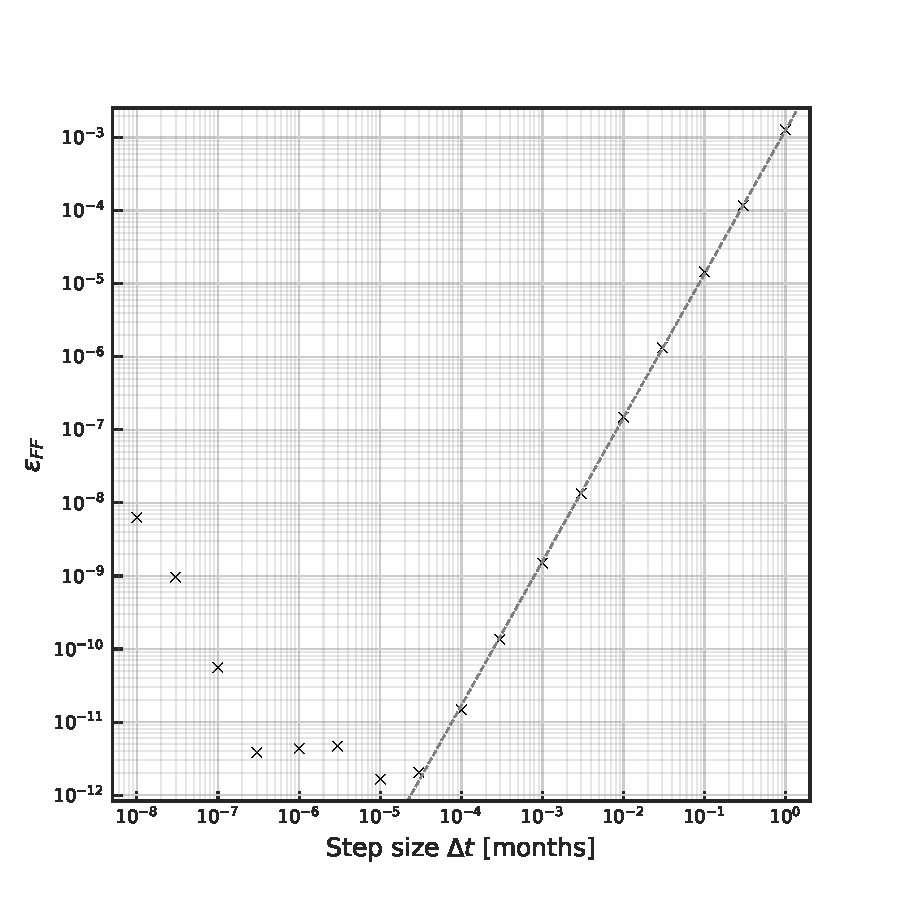
\includegraphics[height=0.9\textheight]{../figures/Global_error_ffwdmethod_max}
    \end{center}
\end{frame}

\begin{frame}
    \frametitle{How do they compare?}
    \begin{center}
        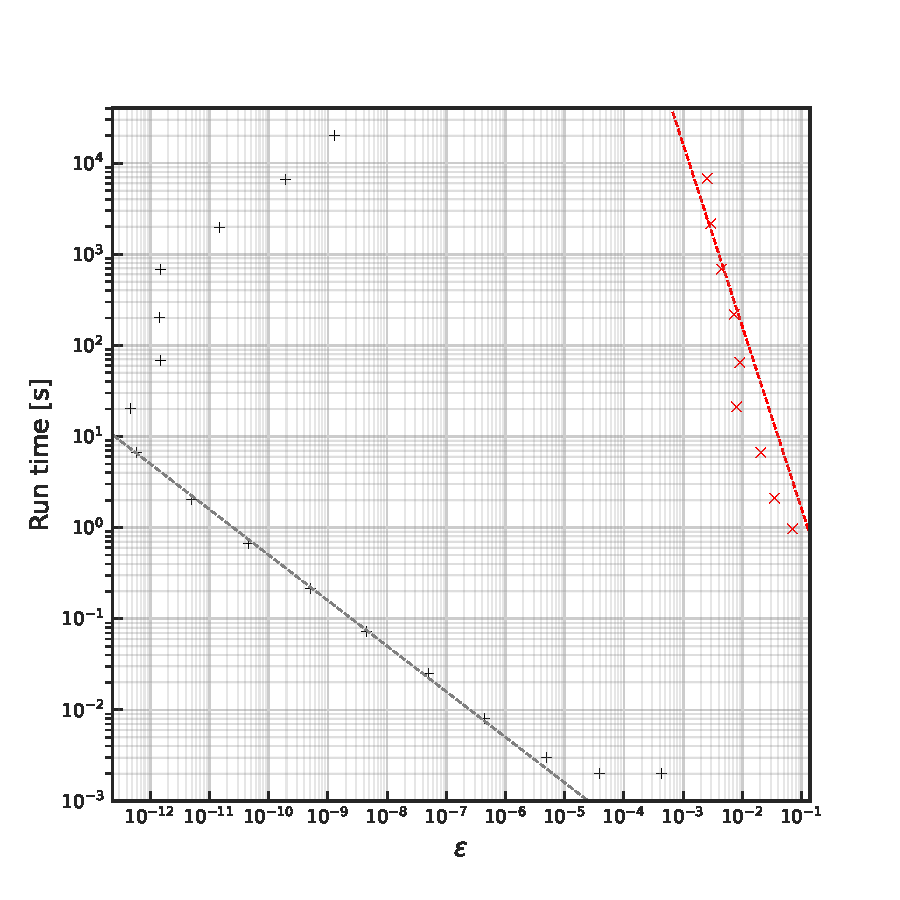
\includegraphics[height=0.9\textheight]{../figures/Error_vs_runtime}
    \end{center}
\end{frame}

\begin{frame}
    \frametitle{Fast forward method}
    Efficiently computing $S_k(a)$ means we can evaluate likelihood functions
    directly, just sampling them.....

    \begin{columns}
        \begin{column}{0.5\textwidth}
        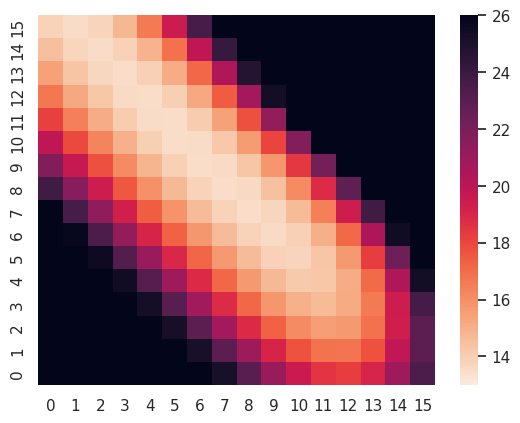
\includegraphics[width=\textwidth]{../figures/raster.png}
        \end{column}
        \begin{column}{0.5\textwidth}
        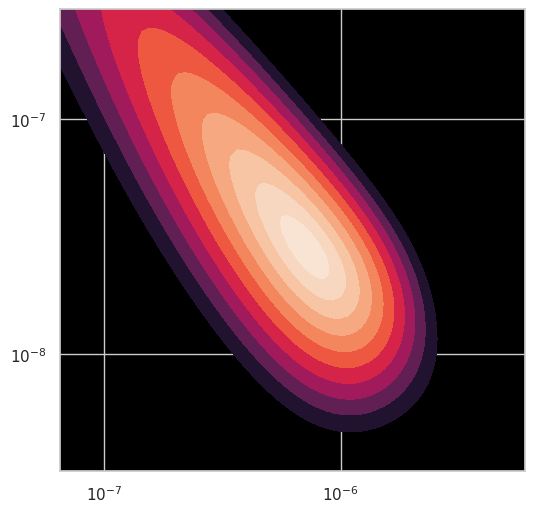
\includegraphics[width=\textwidth]{../figures/contour.png}
        \end{column}
    \end{columns}

\end{frame}


\begin{frame}
    \frametitle{Machine learning with the fast forward method}
    \framesubtitle{The training harness}

    Here, ``machine learning'' means we minimise a function: in this case the
    negative log-likelihood function $-\ln \mathcal{L}$

    \;

    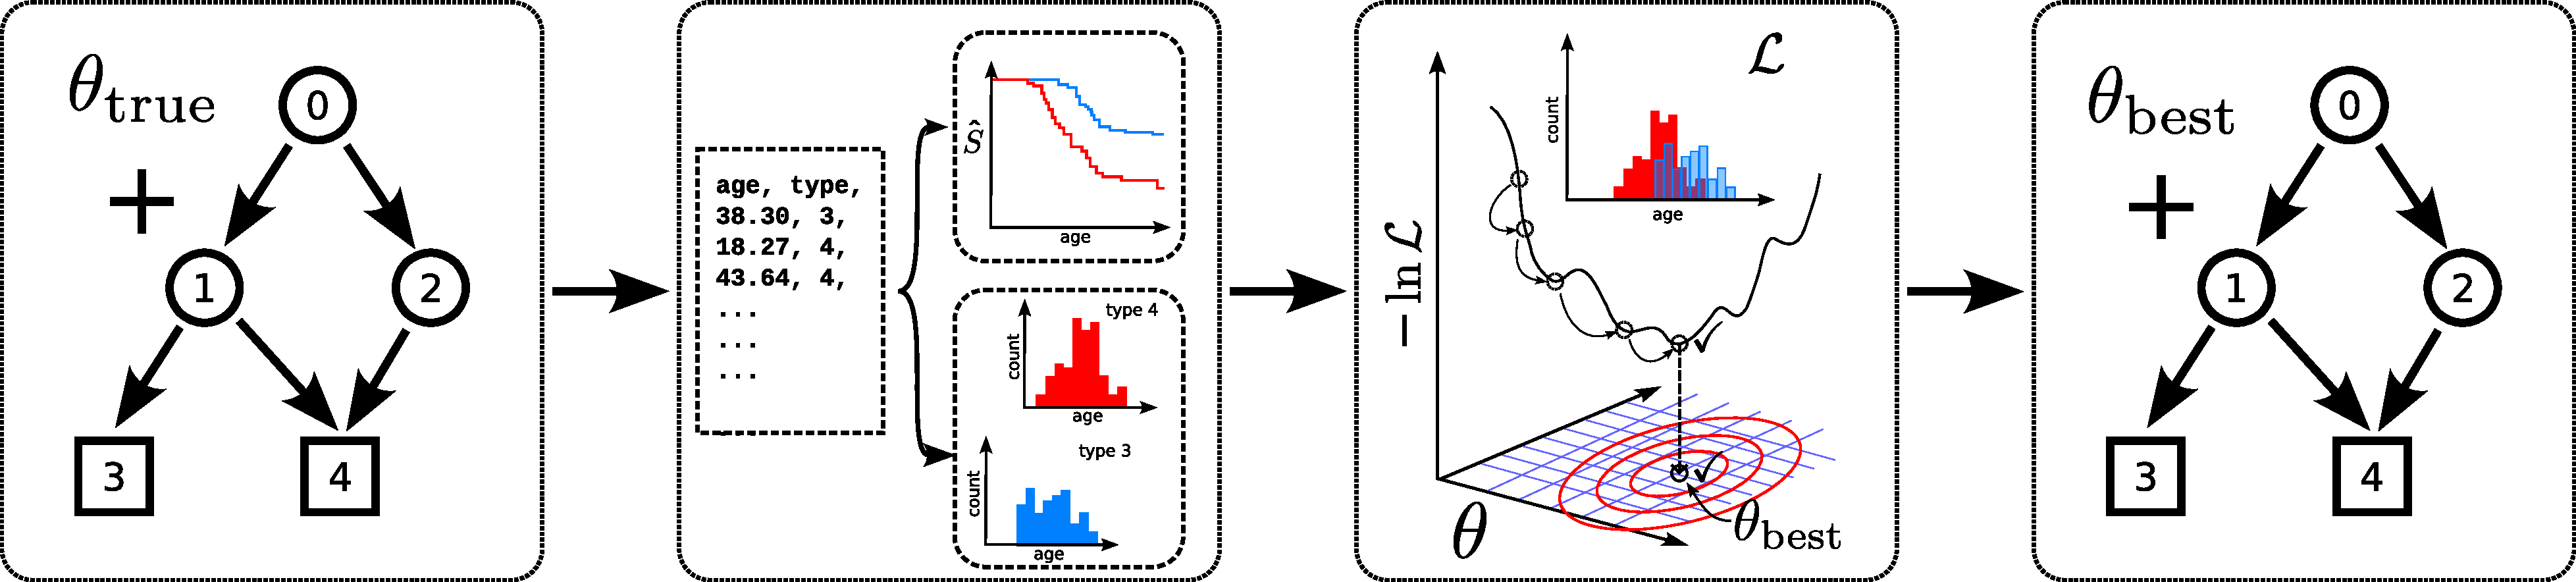
\includegraphics[width=\textwidth]{../figures/flowchart.pdf}

    \;

    generate a simulated study, then find the max. likelihood parameter
    estimates

\end{frame}

\begin{frame}
    \frametitle{Machine learning with the fast forward method}
    \framesubtitle{Parameter inference}
    \begin{columns}
        \begin{column}{0.5\textwidth}
        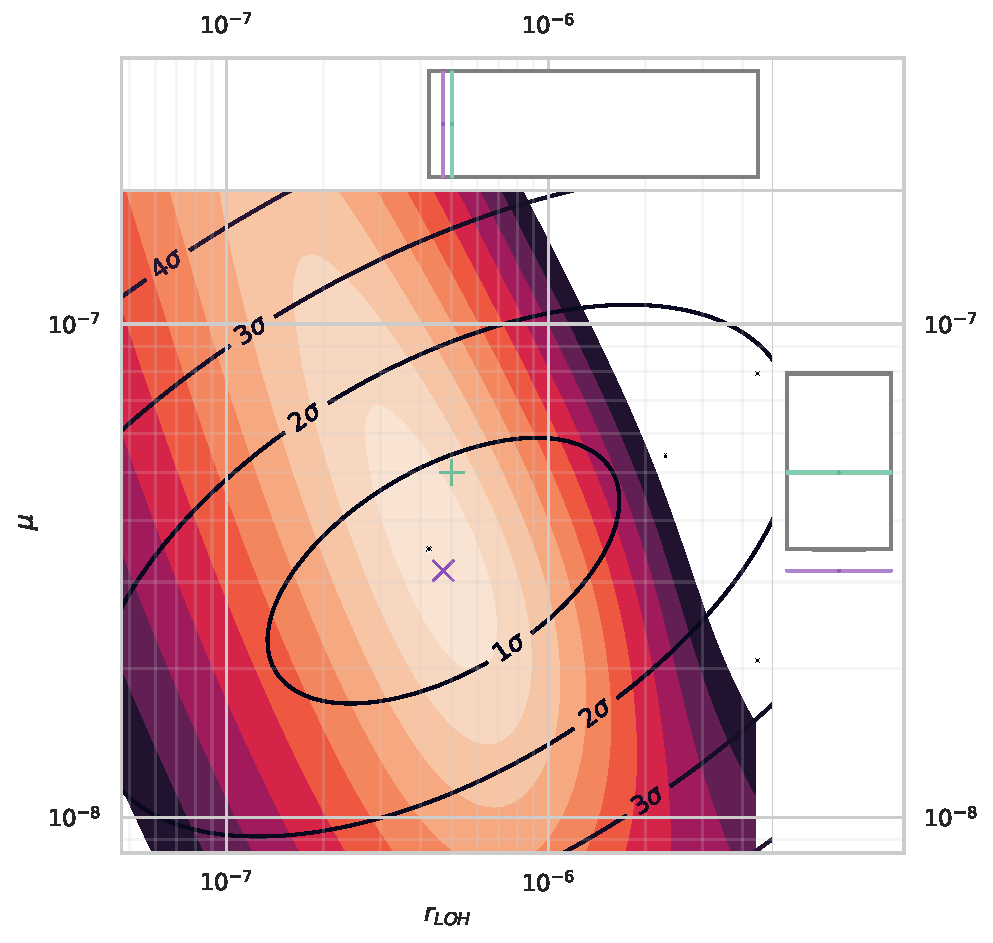
\includegraphics[width=\textwidth]{../figures/scatterplot_floating_mutrates_fixed_32}
        \end{column}
        \begin{column}{0.5\textwidth}
        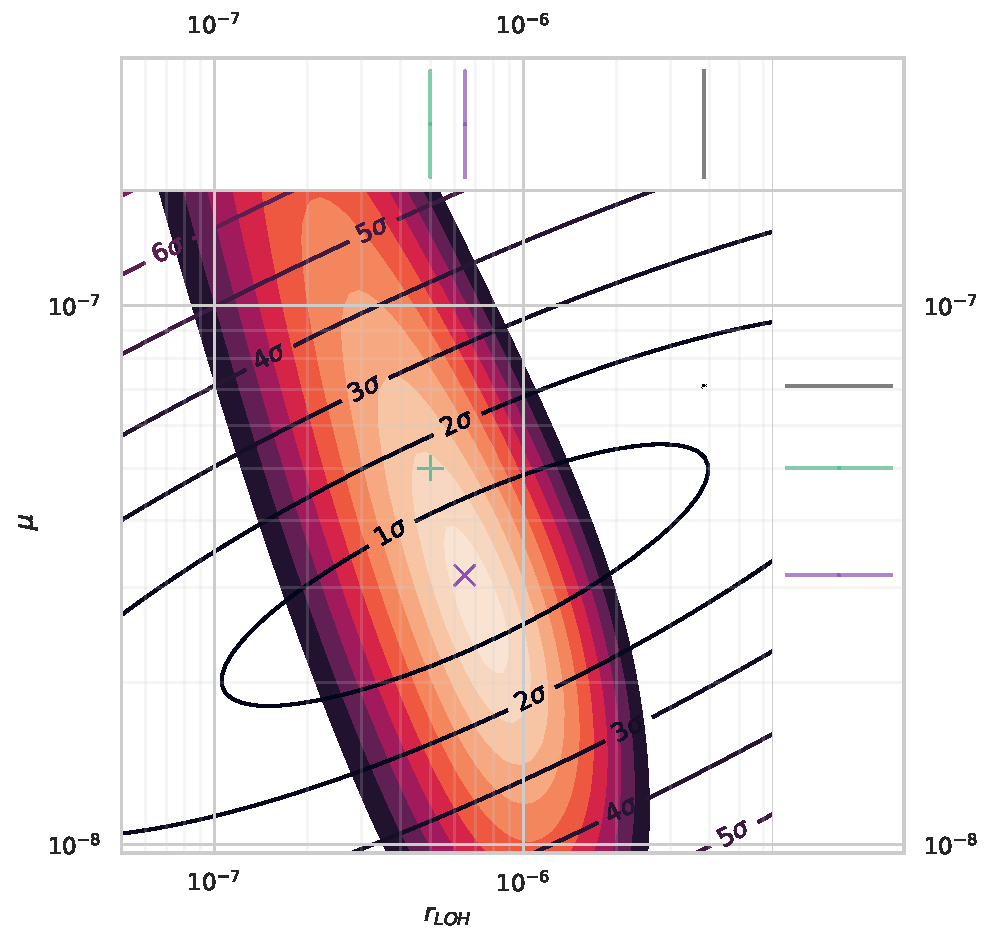
\includegraphics[width=\textwidth]{../figures/scatterplot_floating_mutrates_fixed_100}
        \end{column}
    \end{columns}
\end{frame}

\begin{frame}
    \frametitle{Initial findings from the schwannomatosis project}

    %beamer webm?

    \begin{columns}
        \begin{column}{0.5\textwidth}
        \begin{itemize}
            \item Fitness dis/advantages of single hits to \emph{NF2} tumour suppressor
            practically unidentifiable
            \item Tumour commitment in \emph{NF2}-schwannomatosis occurs very early
            \item \emph{NF2} loss appears to be \emph{sufficient} for a primary
            tumour, with other alterations occurring after 
        \end{itemize}
        \end{column}
        \begin{column}{0.5\textwidth}
        % WEBM
        \movie[label=show3,width=1.0\textwidth,poster,autostart,showcontrols,loop]{}{S5_Video_s1=0.05_s2=0.03_1_1000_swatch1.webm}
        \end{column}
    \end{columns}
\end{frame}

\begin{frame}
    \frametitle{Conclusions and the future}
    \begin{itemize}
        \item Immediate clinical applications \emph{without pharmaceutical
        products}, just better advice about interventions. Both the oncologist
        and patient benefit: clarity about uncertainty/risks is good for
        trust and planning.
        \item There are deep theoretical connections too: Hamiltonian systems
        are v common, I suspect because of irreversibility.
        \item It now appears (as of 2026) that many auto-immune diseases may
        also be caused by clonal expansions too${}^1$
    \end{itemize}

\footnotetext[1]{Pantelis Nicola et al., Nature 654, 131-41 (2026)}
\end{frame}

\begin{frame}
    \frametitle{Acknowledgements}
    \begin{columns}
        \begin{column}{0.5\textwidth}
        
\includegraphics[width=\textwidth]{../figures/cdmrp_logo_03.png}

        DoD(/W) funded this research
        
\includegraphics[width=1.0\textwidth]{../figures/NIHR-MBRC-logo}

        \begin{columns}
            \begin{column}{0.3\textwidth}
            
\includegraphics[width=\textwidth]{../figures/NTUK_RGB}
            \end{column}
            \begin{column}{0.7\textwidth}
            
\includegraphics[width=\textwidth]{../figures/aced_website_header.jpg}
            \end{column}
        \end{columns}

        \end{column}
        \begin{column}{0.5\textwidth}

        % Manchester NHS FT
        
\includegraphics[width=0.75\textwidth]{../figures/MFT-logo}

        
\includegraphics[width=0.3\textwidth]{../figures/W-Logo_Purple1}

        The University of Washington
        \end{column}
    \end{columns}
    \begin{columns}
        \begin{column}{0.5\textwidth}
        
        \begin{center}
        
\includegraphics[width=\textwidth]{../figures/logo_big.jpg}
        \end{center}

        \end{column}
        \begin{column}{0.5\textwidth}
        All my collaborators...

        \begin{itemize}
            \item Vivien Holmes (here!)
            \item Miaomiao Gao
            \item Ivana Bo\v{z}i\'{c} (here!)
            \item Gareth Evans
            \item David Wedge
            \item Miriam Smith
            \item Marian Love
            \item Sean Holman
            \item Joshua Hellier
        \end{itemize}

        \end{column}
    \end{columns}
    % UoM
    % UW
    % NHS
\end{frame}

\end{document}
